\documentclass[a4paper,11pt]{book}
%\documentclass[a4paper,11pt,makeidx]{book} <== may need this to generate index

%  makeindex NEMO_book  <== to regenerate the index
%  bibtex    NEMO_book	<== to generate  the bibliography

%\usepackage[french]{babel}
%\usepackage{color}
\usepackage{rotating, graphicx}			           % allows insertion of pictures
%\usepackage{graphics}			                   % allows insertion of pictures
\graphicspath{{Figures/}}                                  % Set global directory for pictures
\DeclareGraphicsExtensions{.pdf,.eps}                      % Use .eps for LaTeX2HTML
%\usepackage{xcolor}                                       % Incompatibility with color -> graphicx
\usepackage[capbesideposition={top,center}]{floatrow}      % allows captions
\floatsetup[table]{style=plaintop}                         % beside pictures
\usepackage[margin=10pt,font={small},                      % Gives small font for captions
labelsep=colon,labelfont={bf}]{caption}                    %
\usepackage{enumitem}                                      % allows non-bold description items
\usepackage{longtable}                                     % allows multipage tables
%\usepackage{colortbl}                                     % gives coloured panels behind table columns

%hyperref
\usepackage[pdftitle={NEMO ocean engine},pdfauthor={Gurvan Madec},pdfstartview=FitH,
bookmarks=true,bookmarksopen=true,breaklinks=true,colorlinks=true,
linkcolor=blue,anchorcolor=blue,citecolor=blue,filecolor=blue,menucolor=blue,urlcolor=blue]{hyperref}
% pdfsubject={The preprint document class
%   elsart},% pdfkeywords={diapycnal diffusion,numerical mixing,z-level models},%%  usage of exteranl hyperlink :  \href{mailto:my_address@wikibooks.org}{my\_address@wikibooks.org}
%                                                 \url{http://www.wikibooks.org}
%                                     or         \href{http://www.wikibooks.org}{wikibooks home}


%%%% page styles etc................
\usepackage{fancyhdr}
\pagestyle{fancy}
% with this we ensure that the chapter and section
% headings are in lowercase.
\renewcommand{\chaptermark}[1]{\markboth{#1}{}}
\renewcommand{\sectionmark}[1]{\markright{\thesection.\ #1}}
\fancyhf{}             % delete current setting for header and footer
\fancyhead[LE,RO]{\bfseries\thepage}
\fancyhead[LO]{\bfseries\hspace{-0em}\rightmark}
\fancyhead[RE]{\bfseries\leftmark}
\renewcommand{\headrulewidth}{0.5pt}
\renewcommand{\footrulewidth}{0pt  }
\addtolength{\headheight}{2.6pt}   % make space for the rule
%\addtolength{\headheight}{1.6pt}   % make space for the rule
% get rid of headers on plain pages
\fancypagestyle{plain}{\fancyhead{}\renewcommand{\headrulewidth}{0pt}}


%%%%  Section number in Margin.......
% typeset the number of each section in the left margin, with the start of each instance of
% sectional heading text aligned with the left hand edge of  the body text.
\makeatletter
\def\@seccntformat#1{\protect\makebox[0pt][r]{\csname the#1\endcsname\quad}}
\makeatother

% Leave blank pages completely empty, w/o header
\makeatletter
\def\cleardoublepage{\clearpage\if@twoside \ifodd\c@page\else
  \hbox{}
  \vspace*{\fill}
  \vspace{\fill}
  \thispagestyle{empty}
  \newpage
  \if@twocolumn\hbox{}\newpage\fi\fi\fi}
\makeatother

%%%% define the chapter  style ................
\usepackage{minitoc}				%In French : \usepackage[french]{minitoc}
%\usepackage{mtcoff}				% invalidate the use of minitocs
\usepackage{fancybox}

\makeatletter
\def\LigneVerticale{\vrule height 5cm depth 2cm\hspace{0.1cm}\relax}
\def\LignesVerticales{%
  \let\LV\LigneVerticale\LV\LV\LV\LV\LV\LV\LV\LV\LV\LV}
\def\GrosCarreAvecUnChiffre#1{%
  \rlap{\vrule height 0.8cm width 1cm depth 0.2cm}%
 \rlap{\hbox to 1cm{\hss\mbox{\color{white} #1}\hss}}%
  \vrule height 0pt width 1cm depth 0pt}
\def\GrosCarreAvecTroisChiffre#1{%
  \rlap{\vrule height 0.8cm width 1.6cm depth 0.2cm}%
 \rlap{\hbox to 1.5cm{\hss\mbox{\color{white} #1}\hss}}%
  \vrule height 0pt width 1cm depth 0pt}

\def\@makechapterhead#1{\hbox{%
   \huge
    \LignesVerticales
    \hspace{-0.5cm}%
    \GrosCarreAvecUnChiffre{\thechapter}
    \hspace{0.2cm}\hbox{#1}%
%    \GrosCarreAvecTroisChiffre{\thechapter}
%    \hspace{1cm}\hbox{#1}%
%}\par\vskip 2cm}
}\par\vskip 1cm}
\def\@makeschapterhead#1{\hbox{%
   \huge
    \LignesVerticales
    %\hspace{0.5cm}%
    \hbox{#1}%
}\par\vskip 2cm}
\makeatother

%\def\thechapter{\Roman{chapter}}   	% chapter number to be Roman


%%%%           Mathematics...............
%\documentclass{amsart}
\usepackage{xspace}                              % helpd ensure correct spacing after macros
\usepackage{latexsym,amssymb,amsmath}
\allowdisplaybreaks[1]				% allow page breaks in the middle of equations
\usepackage{TexFiles/Styles/math_abbrev}    % use maths shortcuts

\usepackage{times}			 	 % use times font for text
%\usepackage{mathtime}                          % font for illustrator to work (belleek fonts )
%\usepackage[latin1]{inputenc}                % allows some unicode removed (agn)


%%% essai commande
\newcommand{\nl}[1]{\texttt{\small{\textcolor{blue}{#1}}}}
\newcommand{\nlv}[1]{\texttt{\footnotesize#1}\xspace}
\newcommand{\smnlv}[1]{\texttt{\scriptsize#1}\xspace}

%%%% namelist & code display................................
\usepackage{alltt,verbatim}  	%%  alltt & verbatim for namelist
% namelists
\newcommand{\namdisplay}[1]{\begin{alltt}{\tiny\verbatiminput{Namelists/#1}}\end{alltt}\vspace{-10pt}}
\newcommand{\namtools}[1]{\begin{alltt}{\tiny\verbatiminput{Namelists/#1}}\end{alltt}\vspace{-10pt}}
% code display
%\newcommand{\codedisplay} [1] {\begin{alltt}{\tiny {\begin{verbatim} {#1}} \end{verbatim}} \end{alltt}      }



%%%% commands for working with text................................
% command to "comment out" portions of text ({} argument) or not ({#1} argument)
\newcommand{\amtcomment}[1]{}   	% command to "commented out" portions of text or not (#1 in argument)
\newcommand{\sgacomment}[1]{}   	% command to "commented out" portions of
\newcommand{\gmcomment}[1]{}   	% command to "commented out" portions of
%                                    				% text that span line breaks
%Red (NR) or Yellow(WARN)
%\newcommand{\NR}   {\colorbox{red}   {#1}}
%\newcommand{\WARN} {\colorbox{yellow}{#1}}



%%% index commands......................
\usepackage{makeidx}
%\usepackage{showidx}				% show the index entry

\newcommand{\mdl}[1]{\textit{#1.F90}\index{Modules!#1}}	%module (mdl)
\newcommand{\rou}[1]{\textit{#1}\index{Routines!#1}}	%module (routine)
\newcommand{\hf}[1]{\textit{#1.h90}\index{h90 file!#1}}	%module (h90 files)
\newcommand{\ngn}[1]{\textit{#1}\index{Namelist Group Name!#1}}	%namelist name (nampar)
\newcommand{\np}[1]{\textit{#1}\index{Namelist variables!#1}}        %namelist variable
\newcommand{\jp}[1]{\textit{#1}\index{Model parameters!#1}}	%model parameter (jp)
\newcommand{\pp}[1]{\textit{#1}\index{Model parameters!#1}} 	%namelist parameter (pp)
\newcommand{\ifile}[1]{\textit{#1.nc  }\index{Input NetCDF files!#1.nc}}	%input NetCDF files (.nc)
\newcommand{\key}[1]{\textbf{key\_#1}\index{CPP keys!key\_#1}}	%key_cpp (key)
\newcommand{\NEMO}{\textit{NEMO}\xspace}	%NEMO (nemo)

%%%%   Bibliography   .............
\usepackage[nottoc,notlof,notlot]{tocbibind}
\usepackage[square,comma]{natbib}
\bibpunct{[}{]}{,}{a}{}{;}                           %suppress "," after "et al."
\providecommand{\bibfont}{\small}

\usepackage{subfiles}                          % Separate compilation of chapters from whole manual
%\newcommand{\onlyinsubfile}[1]{#1}             % New commands for printing parts according to
%\newcommand{\notinsubfile}[1]{}                % the file being compiled
% Commands to use in the documentfile
%\renewcommand{\onlyinsubfile}[1]{}                      % Appears only if chapter   .tex file is compiled
%\renewcommand{\notinsubfile}[1]{#1}                     %    "    ""   "" NEMO_book .tex file is compiled

\DeclareMathAlphabet{\mathpzc}{OT1}{pzc}{m}{it}


\begin{document}

\title{Draft description of NEMO wetting and drying scheme:     29 November 2017 }

\author{ Enda O'Dea, Hedong Liu, Jason Holt, Andrew Coward  and Michael J. Bell  }

%------------------------------------------------------------------------
% End of temporary latex header (to be removed) 
%------------------------------------------------------------------------

% ================================================================
% Chapter Ocean Dynamics (DYN)
% ================================================================
\chapter{Ocean Dynamics (DYN)}
\label{DYN}
\minitoc

% add a figure for  dynvor ens, ene latices

$\ $\newline    % force a new ligne

% ================================================================
% Wetting and drying 
% ================================================================
\section{Wetting and drying }
\label{DYN_wetdry}

There are two main options for wetting and drying code (wd): 
(a) an iterative limiter (il) and (b) a directional limiter (dl). 
The directional limiter is based on the scheme developed by \cite{WarnerEtal13} for ROMS
which was in turn based on ideas developed for POM by \cite{Oey06}. The iterative
limiter is a new scheme.  The iterative limiter is activated by setting $\mathrm{ln\_wd\_il} = \mathrm{.true.}$
and $\mathrm{ln\_wd\_dl} = \mathrm{.false.}$. The directional limiter is activated
by setting $\mathrm{ln\_wd\_dl} = \mathrm{.true.}$ and $\mathrm{ln\_wd\_il} = \mathrm{.false.}$.

\namdisplay{nam_wad}

The following terminology is used. The depth of the topography (positive downwards)
at each $(i,j)$ point is the quantity stored in array $\mathrm{ht\_wd}$ in the NEMO code.
The height of the free surface (positive upwards) is denoted by $ \mathrm{ssh}$. Given the sign
conventions used, the water depth, $h$, is the height of the free surface plus the depth of the
topography (i.e. $\mathrm{ssh} + \mathrm{ht\_wd}$).

Both wd schemes take all points in the domain below a land elevation of $\mathrm{rn\_wdld}$ to be
covered by water. They require the topography specified with a model
configuration to have negative depths at points where the land is higher than the
topography's reference sea-level. The vertical grid in NEMO is normally computed relative to an
initial state with zero sea surface height elevation. 
The user can choose to compute the vertical grid and heights in the model relative to 
a non-zero reference height for the free surface. This choice affects the calculation of the metrics and depths
(i.e. the $\mathrm{e3t\_0, ht\_0}$ etc. arrays). 

Points where the water depth is less than $\mathrm{rn\_wdmin1}$ are interpreted as ``dry''. 
$\mathrm{rn\_wdmin1}$ is usually chosen to be of order $0.05$m but extreme topographies 
with very steep slopes require larger values for normal choices of time-step. 

Both versions of the code have been tested in six test cases provided in the WAD\_TEST\_CASES configuration
and in ``realistic'' configurations covering parts of the north-west European shelf. 
All these configurations have used pure sigma coordinates. It is expected that
the wetting and drying code will work in domains with more general s-coordinates provided
the coordinates are pure sigma in the region where wetting and drying actually occurs.  

The next sub-section descrbies the directional limiter and the following sub-section the iterative limiter. 
The final sub-section covers some additional considerations that are relevant to both schemes. 

%-----------------------------------------------------------------------------------------
%   Iterative limiters
%-----------------------------------------------------------------------------------------
\subsection   [Directional limiter (\textit{wet\_dry})]
			{Directional limiter (\mdl{wet\_dry})}
\label{DYN_wd_directional_limiter}

The principal idea of the directional limiter is that 
water should not be allowed to flow out of a dry tracer cell (i.e. one whose water depth is less than rn\_wdmin1).

All the changes associated with this option are made to the barotropic solver for the non-linear 
free surface code within dynspg\_ts. 
On each barotropic sub-step the scheme determines the direction of the flow across each face of all the tracer cells
and sets the flux across the face to zero when the flux is from a dry tracer cell. This prevents cells
whose depth is rn\_wdmin1 or less from drying out further. The scheme does not force $h$ (the water depth) at tracer cells
to be at least the minimum depth and hence is able to conserve mass / volume. 

The flux across each $u$-face of a tracer cell is multiplied by a factor zuwdmask (an array which depends on ji and jj). 
If the user sets ln\_wd\_dl\_ramp = .False. then zuwdmask is 1 when the
flux is from a cell with water depth greater than rn\_wdmin1 and 0 otherwise. If the user sets
ln\_wd\_dl\_ramp = .True. the flux across the face is ramped down as the water depth decreases
from 2 * rn\_wdmin1 to rn\_wdmin1. The use of this ramp reduced grid-scale noise in idealised test cases. 

At the point where the flux across a $u$-face is multiplied by zuwdmask , we have chosen
also to multiply the corresponding velocity on the ``now'' step at that face by zuwdmask. We could have
chosen not to do that and to allow fairly large velocities to occur in these ``dry'' cells. 
The rationale for setting the velocity to zero is that it is the momentum equations that are being solved
and the total momentum of the upstream cell (treating it as a finite volume) should be considered
to be its depth times its velocity. This depth is considered to be zero at ``dry'' $u$-points consistent with its 
treatment in the calculation of the flux of mass across the cell face.         

\cite{WarnerEtal13} state that in their scheme the velocity masks at the cell faces for the baroclinic 
timesteps are set to 0 or 1 depending on whether the average of the masks over the barotropic sub-steps is respectively less than 
or greater than 0.5. That scheme does not conserve tracers in integrations started from constant tracer
fields (tracers independent of $x$, $y$ and $z$). Our scheme conserves constant tracers because
the velocities used at the tracer cell faces on the baroclinic timesteps are carefully calculated by dynspg\_ts
to equal their mean value during the barotropic steps. If the user sets ln\_wd\_dl\_bc = .True., the
baroclinic velocities are also multiplied by a suitably weighted average of zuwdmask.      
     
%-----------------------------------------------------------------------------------------
%   Iterative limiters
%-----------------------------------------------------------------------------------------
\subsection   [Iterative limiter (\textit{wet\_dry})]
			{Iterative limiter (\mdl{wet\_dry})}
\label{DYN_wd_iterative_limiter}

\subsubsection [Iterative flux limiter (\textit{wet\_dry})]
			{Iterative flux limiter (\mdl{wet\_dry})}
\label{DYN_wd_il_spg_limiter}

The iterative limiter modifies the fluxes across the faces of cells that are either already ``dry''
or may become dry within the next time-step using an iterative method. 

The flux limiter for the barotropic flow (devised by Hedong Liu) can be understood as follows: 

The continuity equation for the total water depth in a column 
\begin{equation} \label{dyn_wd_continuity}
 \frac{\partial h}{\partial t} + \mathbf{\nabla.}(h\mathbf{u}) = 0 .
\end{equation} 
can be written in discrete form  as  

\begin{align} \label{dyn_wd_continuity_2}
\frac{e_1 e_2}{\Delta t} ( h_{i,j}(t_{n+1}) - h_{i,j}(t_e) ) 
&= - ( \mathrm{flxu}_{i+1,j} - \mathrm{flxu}_{i,j}  + \mathrm{flxv}_{i,j+1} - \mathrm{flxv}_{i,j} ) \\
&= \mathrm{zzflx}_{i,j} .
\end{align} 

In the above $h$ is the depth of the water in the column at point $(i,j)$,
$\mathrm{flxu}_{i+1,j}$ is the flux out of the ``eastern'' face of the cell and
$\mathrm{flxv}_{i,j+1}$ the flux out of the ``northern'' face of the cell; $t_{n+1}$ is
the new timestep, $t_e$ is the old timestep (either $t_b$ or $t_n$) and $ \Delta t =
t_{n+1} - t_e$; $e_1 e_2$ is the area of the tracer cells centred at $(i,j)$ and
$\mathrm{zzflx}$ is the sum of the fluxes through all the faces.

The flux limiter splits the flux $\mathrm{zzflx}$ into fluxes that are out of the cell
(zzflxp) and fluxes that are into the cell (zzflxn).  Clearly

\begin{equation} \label{dyn_wd_zzflx_p_n_1}
\mathrm{zzflx}_{i,j} = \mathrm{zzflxp}_{i,j} + \mathrm{zzflxn}_{i,j} .  
\end{equation} 

The flux limiter iteratively adjusts the fluxes $\mathrm{flxu}$ and $\mathrm{flxv}$ until
none of the cells will ``dry out''. To be precise the fluxes are limited until none of the
cells has water depth less than $\mathrm{rn\_wdmin1}$ on step $n+1$.

Let the fluxes on the $m$th iteration step be denoted by $\mathrm{flxu}^{(m)}$ and
$\mathrm{flxv}^{(m)}$.  Then the adjustment is achieved by seeking a set of coefficients,
$\mathrm{zcoef}_{i,j}^{(m)}$ such that:

\begin{equation} \label{dyn_wd_continuity_coef}
\begin{split}
\mathrm{zzflxp}^{(m)}_{i,j} =& \mathrm{zcoef}_{i,j}^{(m)} \mathrm{zzflxp}^{(0)}_{i,j} \\
\mathrm{zzflxn}^{(m)}_{i,j} =& \mathrm{zcoef}_{i,j}^{(m)} \mathrm{zzflxn}^{(0)}_{i,j}
\end{split}
\end{equation} 
 
where the coefficients are $1.0$ generally but can vary between $0.0$ and $1.0$ around
cells that would otherwise dry.

The iteration is initialised by setting

\begin{equation} \label{dyn_wd_zzflx_initial}
\mathrm{zzflxp^{(0)}}_{i,j} = \mathrm{zzflxp}_{i,j} , \quad  \mathrm{zzflxn^{(0)}}_{i,j} = \mathrm{zzflxn}_{i,j} . 
\end{equation} 

The fluxes out of cell $(i,j)$ are updated at the $m+1$th iteration if the depth of the
cell on timestep $t_e$, namely $h_{i,j}(t_e)$, is less than the total flux out of the cell
times the timestep divided by the cell area. Using (\ref{dyn_wd_continuity_2}) this
condition is

\begin{equation} \label{dyn_wd_continuity_if}
h_{i,j}(t_e)  - \mathrm{rn\_wdmin1} <  \frac{\Delta t}{e_1 e_2} ( \mathrm{zzflxp}^{(m)}_{i,j} + \mathrm{zzflxn}^{(m)}_{i,j} ) .
\end{equation} 

Rearranging (\ref{dyn_wd_continuity_if}) we can obtain an expression for the maximum
outward flux that can be allowed and still maintain the minimum wet depth:

\begin{equation} \label{dyn_wd_max_flux}
\begin{split}
\mathrm{zzflxp}^{(m+1)}_{i,j} = \Big[ (h_{i,j}(t_e) & - \mathrm{rn\_wdmin1} - \mathrm{rn\_wdmin2})  \frac{e_1 e_2}{\Delta t} \phantom{]} \\
\phantom{[} & -  \mathrm{zzflxn}^{(m)}_{i,j} \Big]
\end{split}
\end{equation}

Note a small tolerance ($\mathrm{rn\_wdmin2}$) has been introduced here {\it [Q: Why is
this necessary/desirable?]}. Substituting from (\ref{dyn_wd_continuity_coef}) gives an
expression for the coefficient needed to multiply the outward flux at this cell in order
to avoid drying. 

\begin{equation} \label{dyn_wd_continuity_nxtcoef}
\begin{split}
\mathrm{zcoef}^{(m+1)}_{i,j} = \Big[ (h_{i,j}(t_e) & - \mathrm{rn\_wdmin1} - \mathrm{rn\_wdmin2})  \frac{e_1 e_2}{\Delta t} \phantom{]} \\
\phantom{[} & -  \mathrm{zzflxn}^{(m)}_{i,j} \Big] \frac{1}{ \mathrm{zzflxp}^{(0)}_{i,j} } 
\end{split}
\end{equation} 

Only the outward flux components are altered but, of course, outward fluxes from one cell
are inward fluxes to adjacent cells and the balance in these cells may need subsequent
adjustment; hence the iterative nature of this scheme.  Note, for example, that the flux
across the ``eastern'' face of the $(i,j)$th cell is only updated at the $m+1$th iteration
if that flux at the $m$th iteration is out of the $(i,j)$th cell. If that is the case then
the flux across that face is into the $(i+1,j)$ cell and that flux will not be updated by
the calculation for the $(i+1,j)$th cell. In this sense the updates to the fluxes across
the faces of the cells do not ``compete'' (they do not over-write each other) and one
would expect the scheme to converge relatively quickly. The scheme is flux based so
conserves mass. It also conserves constant tracers for the same reason that the 
directional limiter does.  


%----------------------------------------------------------------------------------------
%      Surface pressure gradients
%----------------------------------------------------------------------------------------
\subsubsection   [Modification of surface pressure gradients (\textit{dynhpg})]
			{Modification of surface pressure gradients (\mdl{dynhpg})}
\label{DYN_wd_il_spg}

At ``dry'' points the water depth is usually close to $\mathrm{rn\_wdmin1}$. If the
topography is sloping at these points the sea-surface will have a similar slope and there
will hence be very large horizontal pressure gradients at these points. The WAD modifies
the magnitude but not the sign of the surface pressure gradients (zhpi and zhpj) at such
points by mulitplying them by positive factors (zcpx and zcpy respectively) that lie
between $0$ and $1$.

We describe how the scheme works for the ``eastward'' pressure gradient, zhpi, calculated
at the $(i,j)$th $u$-point. The scheme uses the ht\_wd depths and surface heights at the
neighbouring $(i+1,j)$ and $(i,j)$ tracer points.  zcpx is calculated using two logicals
variables, $\mathrm{ll\_tmp1}$ and $\mathrm{ll\_tmp2}$ which are evaluated for each grid
column.  The three possible combinations are illustrated in figure \ref{Fig_WAD_dynhpg}.
%>>>>>>>>>>>>>>>>>>>>>>>>>>>>>>>>>>>>>>>>>>>>
\begin{figure}[!ht] \begin{center}
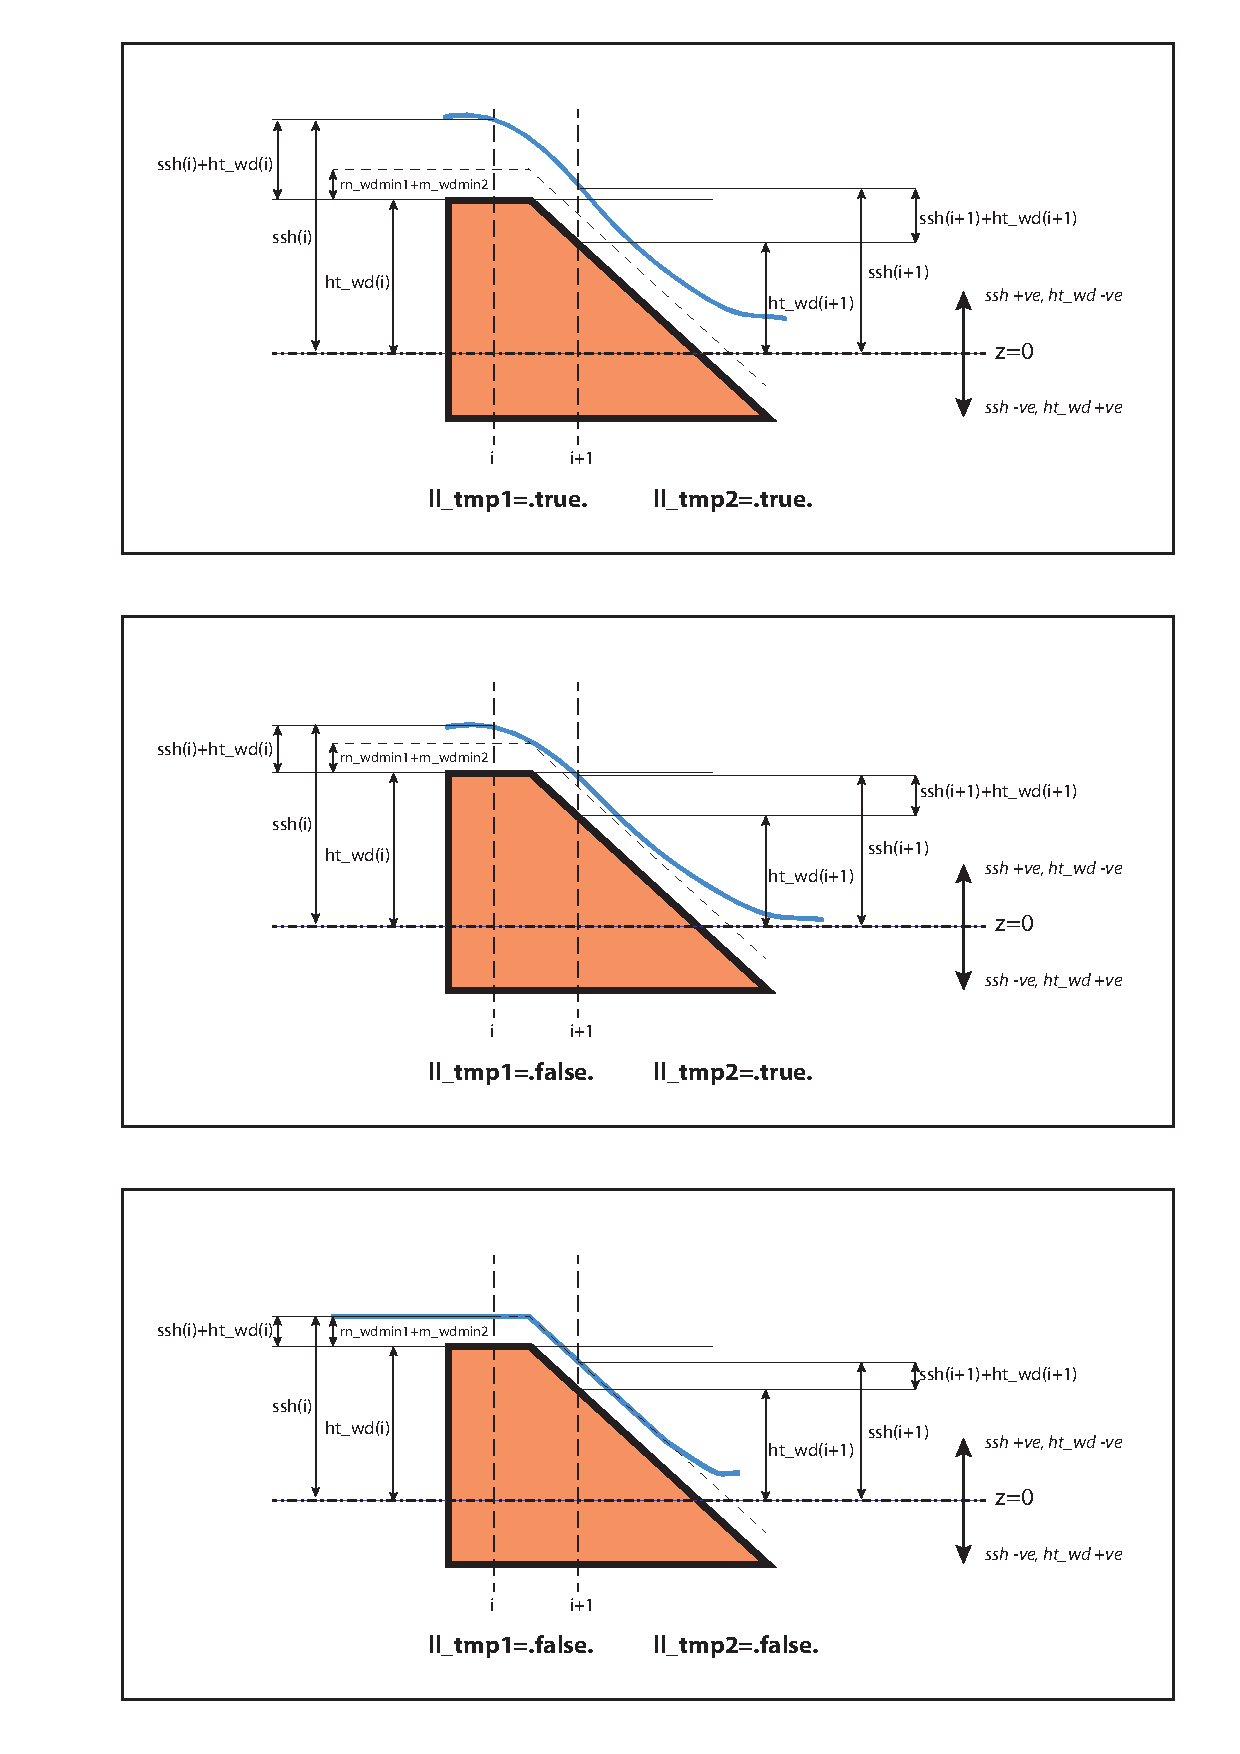
\includegraphics[width=0.8\textwidth]{Fig_WAD_dynhpg}
\caption{ \label{Fig_WAD_dynhpg}
Illustrations of the three possible combinations of the logical variables controlling the 
limiting of the horizontal pressure gradient in wetting and drying regimes}
\end{center}\end{figure}
%>>>>>>>>>>>>>>>>>>>>>>>>>>>>>>>>>>>>>>>>>>>>

The first logical, $\mathrm{ll\_tmp1}$, is set to true if and only if the water depth at
both neighbouring points is greater than $\mathrm{rn\_wdmin1} + \mathrm{rn\_wdmin2}$ and
the minimum height of the sea surface at the two points is greater than the maximum height
of the topography at the two points:

\begin{equation} \label{dyn_ll_tmp1}
\begin{split}
\mathrm{ll\_tmp1}  = & \mathrm{MIN(sshn(ji,jj), sshn(ji+1,jj))} > \\
                     & \quad \mathrm{MAX(-ht\_wd(ji,jj), -ht\_wd(ji+1,jj))\  .and.} \\
& \mathrm{MAX(sshn(ji,jj) + ht\_wd(ji,jj),} \\
& \mathrm{\phantom{MAX(}sshn(ji+1,jj) + ht\_wd(ji+1,jj))} >\\
& \quad\quad\mathrm{rn\_wdmin1 + rn\_wdmin2 }
\end{split}
\end{equation} 

The second logical, $\mathrm{ll\_tmp2}$, is set to true if and only if the maximum height
of the sea surface at the two points is greater than the maximum height of the topography
at the two points plus $\mathrm{rn\_wdmin1} + \mathrm{rn\_wdmin2}$

\begin{equation} \label{dyn_ll_tmp2}
\begin{split}
\mathrm{ ll\_tmp2 } = & \mathrm{( ABS( sshn(ji,jj) - sshn(ji+1,jj) ) > 1.E-12 )\ .AND.}\\
& \mathrm{( MAX(sshn(ji,jj), sshn(ji+1,jj)) > } \\
& \mathrm{\phantom{(} MAX(-ht\_wd(ji,jj), -ht\_wd(ji+1,jj)) + rn\_wdmin1 + rn\_wdmin2}) .
\end{split}
\end{equation} 

If $\mathrm{ll\_tmp1}$ is true then the surface pressure gradient, zhpi at the $(i,j)$
point is unmodified. If both logicals are false zhpi is set to zero.

If $\mathrm{ll\_tmp1}$ is true and $\mathrm{ll\_tmp2}$ is false then the surface pressure
gradient is multiplied through by zcpx which is the absolute value of the difference in
the water depths at the two points divided by the difference in the surface heights at the
two points. Thus the sign of the sea surface height gradient is retained but the magnitude
of the pressure force is determined by the difference in water depths rather than the
difference in surface height between the two points. Note that dividing by the difference
between the sea surface heights can be problematic if the heights approach parity. An
additional condition is applied to $\mathrm{ ll\_tmp2 }$ to ensure it is .false. in such
conditions.

\subsection   [Additional considerations (\textit{usrdef\_zgr})]
			{Additional considerations (\mdl{usrdef\_zgr})}
\label{WAD_additional}

In the very shallow water where wetting and drying occurs the parametrisation of 
bottom drag is clearly very important. In order to promote stability  
it is sometimes useful to calculate the bottom drag using an implicit time-stepping approach.  

Suitable specifcation of the surface heat flux in wetting and drying domains in forced and 
coupled simulations needs further consideration. In order to prevent freezing or boiling
in uncoupled integrations the net surface heat fluxes need to be appropriately limited.  
 
%----------------------------------------------------------------------------------------
%      The WAD test cases
%----------------------------------------------------------------------------------------
\subsection   [The WAD test cases (\textit{usrdef\_zgr})]
			{The WAD test cases (\mdl{usrdef\_zgr})}
\label{WAD_test_cases}

This section contains details of the seven test cases that can be run as part of the
WAD\_TEST\_CASES configuration. All the test cases are shallow (less than 10m deep),
basins or channels with 4m high walls and some of topography that can wet and dry up to
2.5m above sea-level. The horizontal grid is uniform with a 1km resolution and measures
52km by 34km. These dimensions are determined by a combination of code in the
\mdl{usrdef\_nam} module located in the WAD\_TEST\_CASES/MY\_SRC directory and setting
read in from the namusr\_def namelist. The first six test cases are closed systems with no
rotation or external forcing and motion is simply initiated by an initial ssh slope. The
seventh test case introduces and open boundary at the right-hand end of the channel which
is forced with sinousoidally varying ssh and barotropic velocities.

\namdisplay{nam_wad_usr}

The $\mathrm{nn\_wad\_test}$ parameter can takes values 1 to 7 and it is this parameter
that determines which of the test cases will be run. Most cases can be run with the
default settings but the simple linear slope cases (tests 1 and 5) can be run with lower
values of $\mathrm{rn\_wdmin1}$. Any recommended changes to the default namelist settings
will be stated in the individual subsections.

Test case 7 requires additional {\tt namelist\_cfg} changes to activate the open boundary
and lengthen the duration of the run (in order to demonstrate the full forcing cycle).
There is also a simple python script which needs to be run in order to generate the
boundary forcing files.  Full details are given in subsection (\ref{WAD_test_case7}).

\clearpage
\subsubsection [WAD test case 1 : A simple linear slope]
                    {WAD test case 1 : A simple linear slope}
\label{WAD_test_case1}

The first test case is a simple linear slope (in the x-direction, uniform in y) with an
adverse SSH gradient that, when released, creates a surge up the slope. The parameters are
chosen such that the surge rises above sea-level before falling back and oscillating
towards an equilibrium position. This case can be run with $\mathrm{rn\_wdmin1}$ values as
low as 0.075m. I.e. the following change may be made to the default values in {\tt
namelist\_cfg} (for this test only):

\namdisplay{nam_wad_tc1}

%>>>>>>>>>>>>>>>>>>>>>>>>>>>>>>>>>>>>>>>>>>>>
\begin{figure}[htb] \begin{center}
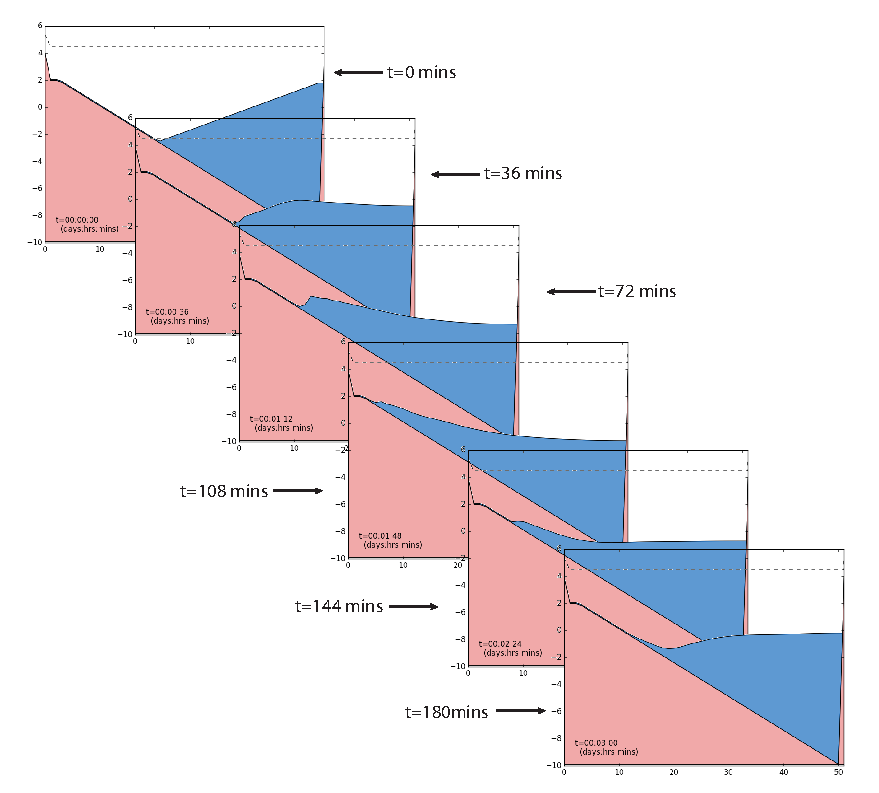
\includegraphics[width=0.8\textwidth]{Fig_WAD_TC1}
\caption{ \label{Fig_WAD_TC1}
The evolution of the sea surface height in WAD\_TEST\_CASE 1 from the initial state (t=0)
over the first three hours of simulation. Note that in this time-frame the resultant surge
reaches to nearly 2m above sea-level before retreating.}
\end{center}\end{figure}
%>>>>>>>>>>>>>>>>>>>>>>>>>>>>>>>>>>>>>>>>>>>>

\clearpage
\subsubsection [WAD test case 2 : A parabolic channel ]
                    {WAD test case 2 : A parabolic channel}
\label{WAD_test_case2}

The second and third test cases use a closed channel which is parabolic in x and uniform
in y.  Test case 2 uses a gentler initial SSH slope which nevertheless demonstrates the
ability to wet and dry on both sides of the channel. This solution requires values of
$\mathrm{rn\_wdmin1}$ at least 0.3m ({\it Q.: A function of the maximum topographic
slope?})

\namdisplay{nam_wad_tc2}

%>>>>>>>>>>>>>>>>>>>>>>>>>>>>>>>>>>>>>>>>>>>>
\begin{figure}[htb] \begin{center}
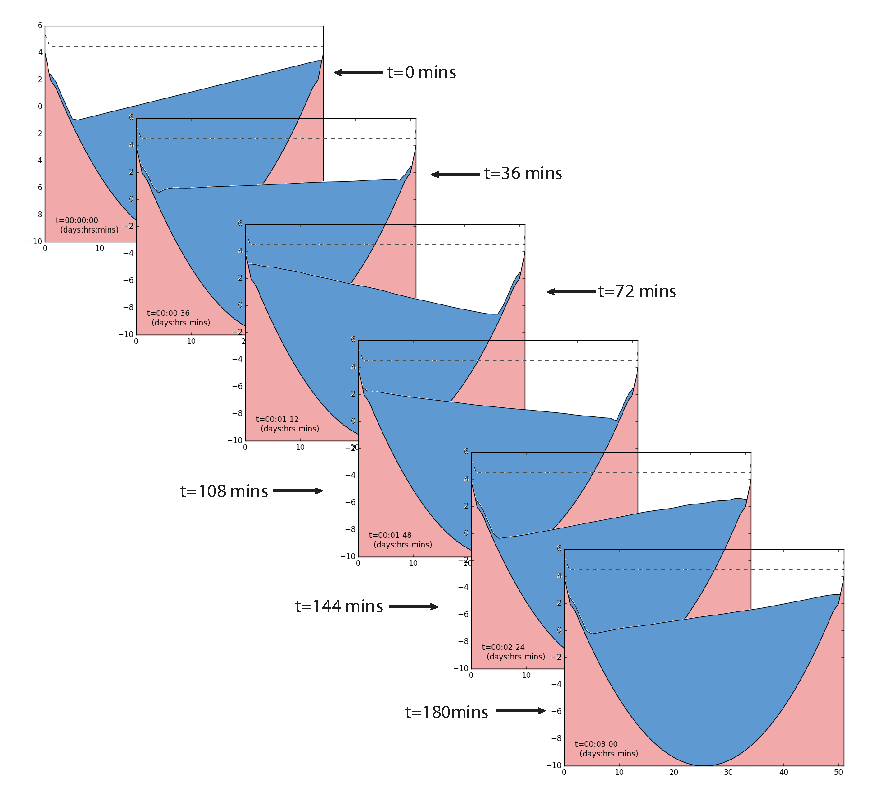
\includegraphics[width=0.8\textwidth]{Fig_WAD_TC2}
\caption{ \label{Fig_WAD_TC2}
The evolution of the sea surface height in WAD\_TEST\_CASE 2 from the initial state (t=0)
over the first three hours of simulation. Note that in this time-frame the resultant sloshing
causes wetting and drying on both sides of the parabolic channel.}
\end{center}\end{figure}
%>>>>>>>>>>>>>>>>>>>>>>>>>>>>>>>>>>>>>>>>>>>>

\clearpage
\subsubsection [WAD test case 3 : A parabolic channel (extreme slope) ]
                    {WAD test case 3 : A parabolic channel (extreme slope)}
\label{WAD_test_case3}

Similar to test case 2 but with a steeper initial SSH slope. The solution is similar but more vigorous.

\namdisplay{nam_wad_tc3}

%>>>>>>>>>>>>>>>>>>>>>>>>>>>>>>>>>>>>>>>>>>>>
\begin{figure}[htb] \begin{center}
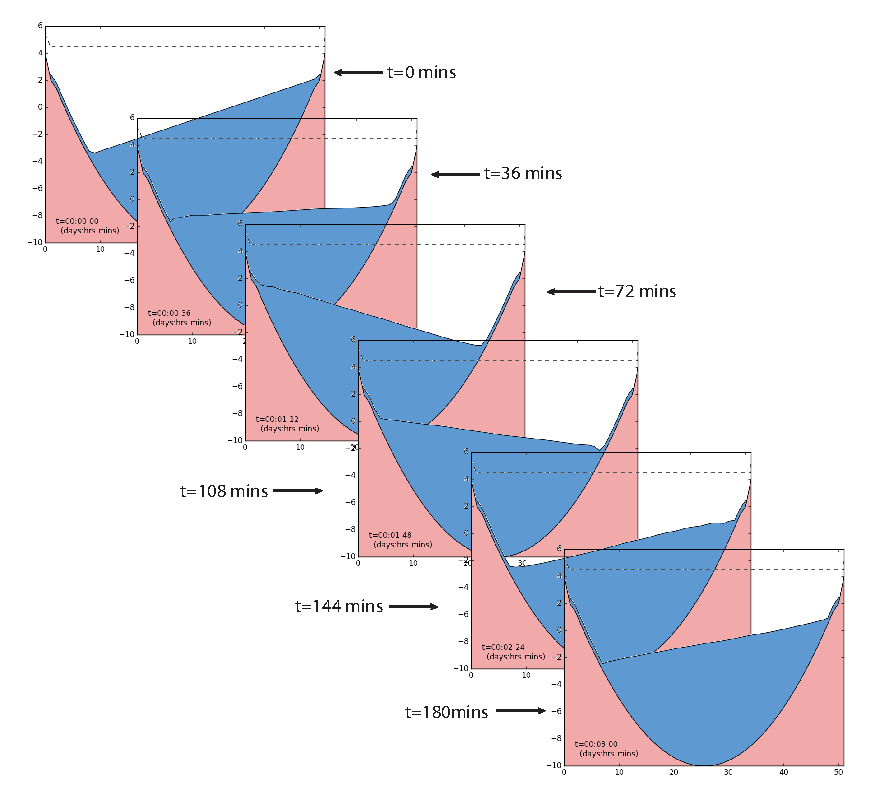
\includegraphics[width=0.8\textwidth]{Fig_WAD_TC3}
\caption{ \label{Fig_WAD_TC3}
The evolution of the sea surface height in WAD\_TEST\_CASE 3 from the initial state (t=0)
over the first three hours of simulation. Note that in this time-frame the resultant sloshing
causes wetting and drying on both sides of the parabolic channel.}
\end{center}\end{figure}
%>>>>>>>>>>>>>>>>>>>>>>>>>>>>>>>>>>>>>>>>>>>>

\clearpage
\subsubsection [WAD test case 4 : A parabolic bowl ]
                    {WAD test case 4 : A parabolic bowl}
\label{WAD_test_case4}

Test case 4 includes variation in the y-direction in the form of a parabolic bowl. The
initial condition is now a raised bulge centred over the bowl. Figure \ref{Fig_WAD_TC4}
shows a cross-section of the SSH in the X-direction but features can be seen to propagate
in all directions and interfere when return paths cross.

\namdisplay{nam_wad_tc4}

%>>>>>>>>>>>>>>>>>>>>>>>>>>>>>>>>>>>>>>>>>>>>
\begin{figure}[htb] \begin{center}
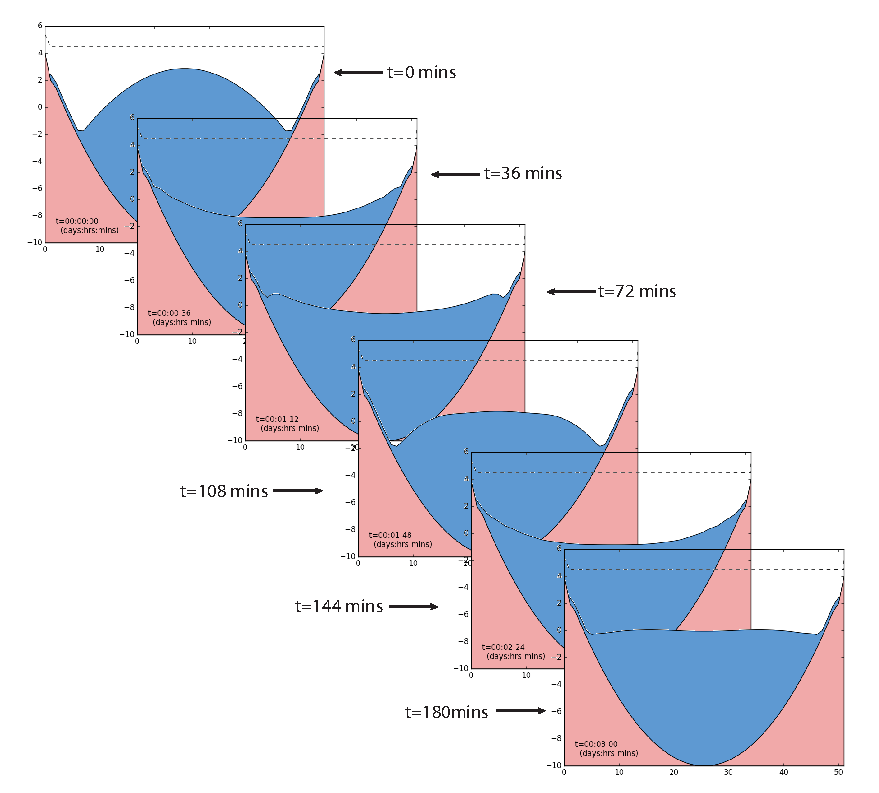
\includegraphics[width=0.8\textwidth]{Fig_WAD_TC4}
\caption{ \label{Fig_WAD_TC4}
The evolution of the sea surface height in WAD\_TEST\_CASE 4 from the initial state (t=0)
over the first three hours of simulation. Note that this test case is a parabolic bowl with
variations occurring in the y-direction too (not shown here).}
\end{center}\end{figure}
%>>>>>>>>>>>>>>>>>>>>>>>>>>>>>>>>>>>>>>>>>>>>

\clearpage
\subsubsection [WAD test case 5 : A double slope with shelf channel ]
                    {WAD test case 5 : A double slope with shelf channel}
\label{WAD_test_case5}

Similar in nature to test case 1 but with a change in slope and a mid-depth shelf.

\namdisplay{nam_wad_tc5}

%>>>>>>>>>>>>>>>>>>>>>>>>>>>>>>>>>>>>>>>>>>>>
\begin{figure}[htb] \begin{center}
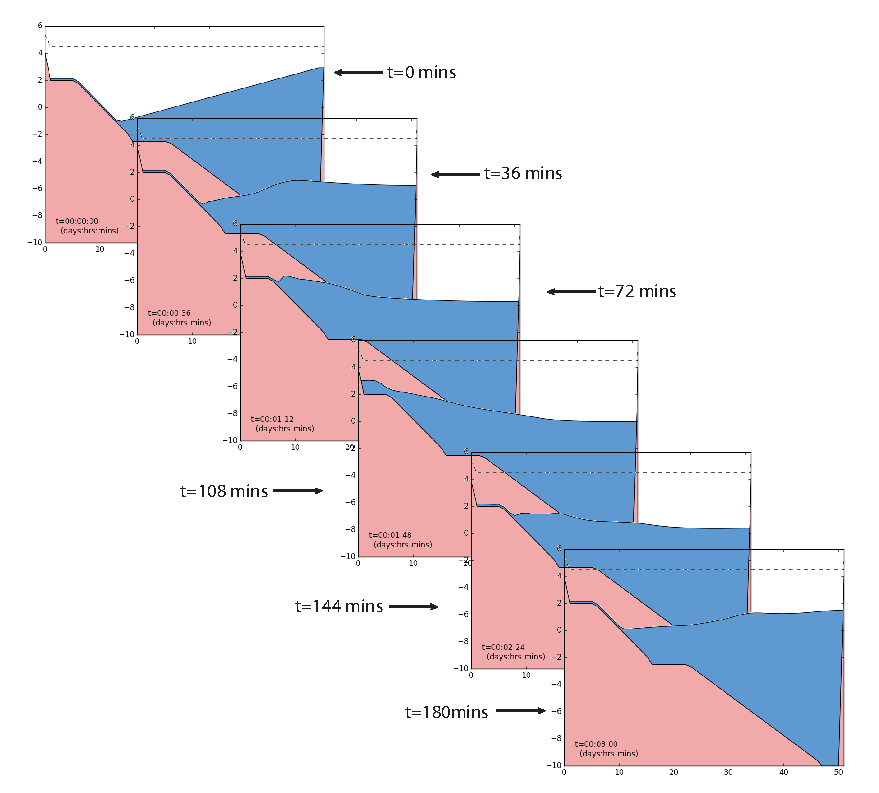
\includegraphics[width=0.8\textwidth]{Fig_WAD_TC5}
\caption{ \label{Fig_WAD_TC5}
The evolution of the sea surface height in WAD\_TEST\_CASE 5 from the initial state (t=0)
over the first three hours of simulation. The surge resulting in this case wets to the full 
depth permitted (2.5m above sea-level) and is only halted by the 4m high side walls.}
\end{center}\end{figure}
%>>>>>>>>>>>>>>>>>>>>>>>>>>>>>>>>>>>>>>>>>>>>

\clearpage
\subsubsection [WAD test case 6 : A parabolic channel with central bar ]
                    {WAD test case 6 : A parabolic channel with central bar}
\label{WAD_test_case6}

Test cases 1 to 5 have all used uniform T and S conditions. The dashed line in each plot
shows the surface salinity along the y=17 line which remains satisfactorily constant. Test
case 6 introduces variation in salinity by taking a parabolic channel divided by a central
bar (gaussian) and using two different salinity values in each half of the channel. This
step change in salinity is initially enforced by the central bar but the bar is
subsequently over-topped after the initial SSH gradient is released. The time series in
this case shows the SSH evolution with the water coloured according to local salinity
values. Encroachment of the high salinity (red) waters into the low salinity (blue) basin
can clearly be seen.

\namdisplay{nam_wad_tc6}

%>>>>>>>>>>>>>>>>>>>>>>>>>>>>>>>>>>>>>>>>>>>>
\begin{figure}[htb] \begin{center}
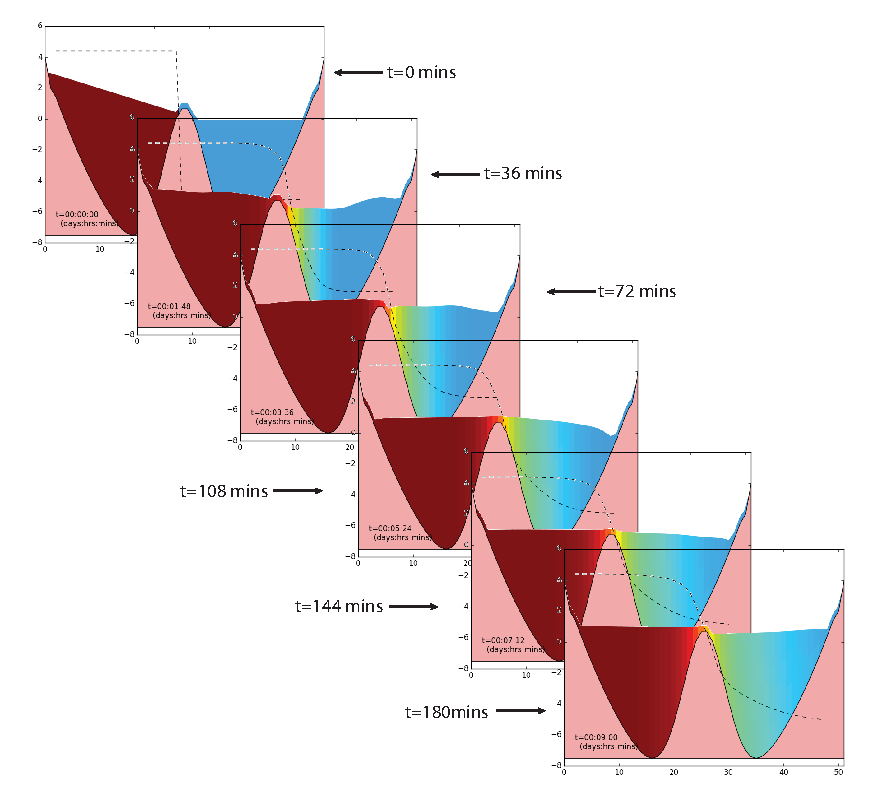
\includegraphics[width=0.8\textwidth]{Fig_WAD_TC6}
\caption{ \label{Fig_WAD_TC6}
The evolution of the sea surface height in WAD\_TEST\_CASE 6 from the initial state (t=0)
over the first three hours of simulation. Water is coloured according to local salinity
values. Encroachment of the high salinity (red) waters into the low salinity (blue) basin
can clearly be seen although the largest influx occurs early in the sequence between the
frames shown.}
\end{center}\end{figure}
%>>>>>>>>>>>>>>>>>>>>>>>>>>>>>>>>>>>>>>>>>>>>

\clearpage
\subsubsection [WAD test case 7 : A double slope with shelf, open-ended channel ]
                    {WAD test case 7 : A double slope with shelf, open-ended channel}
\label{WAD_test_case7}

Similar in nature to test case 5 but with an open boundary forced with a sinusoidally
varying ssh. This test case has been introduced to emulate a typical coastal application
with a tidally forced open boundary. The bathymetry and setup is identical to test case 5
except the right hand end of the channel is now open and has simple ssh and barotropic
velocity boundary conditions applied at the open boundary. Several additional steps and
namelist changes are required to run this test.

\namdisplay{nam_wad_tc7}

In addition, the boundary condition files must be generated using the python script
provided.

\begin{verbatim}
python ./makebdy_tc7.py
\end{verbatim}

will create the following boundary files for this test (assuming a suitably configured
python environment: python2.7 with netCDF4 and numpy):

\begin{verbatim}
  bdyssh_tc7_m12d30.nc   bdyuv_tc7_m12d30.nc
  bdyssh_tc7_m01d01.nc   bdyuv_tc7_m01d01.nc
  bdyssh_tc7_m01d02.nc   bdyuv_tc7_m01d02.nc
  bdyssh_tc7_m01d03.nc   bdyuv_tc7_m01d03.nc
\end{verbatim}

These are sufficient for up to a three day simulation; the script is easily adapted if
longer periods are required.

%>>>>>>>>>>>>>>>>>>>>>>>>>>>>>>>>>>>>>>>>>>>>
\begin{sidewaysfigure}[htb] \begin{center}
\includegraphics[width=0.8\textwidth]{Fig_WAD_TC7}
\caption{ \label{Fig_WAD_TC7}
The evolution of the sea surface height in WAD\_TEST\_CASE 7 from the initial state (t=0)
over the first 24 hours of simulation. After the initial surge the solution settles into a
simulated tidal cycle with an amplitude of 5m. This is enough to repeatedly wet and dry
both shelves.}

\end{center}\end{sidewaysfigure}
%>>>>>>>>>>>>>>>>>>>>>>>>>>>>>>>>>>>>>>>>>>>>


% ================================================================

\bibliographystyle{wileyqj}
\bibliography{references}

\end{document}
